\documentclass[12pt,a4paper,twoside,openright]{report}
\let\openright=\cleardoublepage



%%% Choose a language %%%

\newif\ifEN
\ENtrue   % uncomment this for english
%\ENfalse   % uncomment this for czech

%%% Configuration of the title page %%%

\newif\ifMFF
\MFFtrue % comment this out for the version with a big UK university logo
\def\UKName{Charles University in Prague} %this is used in UK-logo-version
\def\UKFaculty{Faculty of Mathematics and Physics}
\def\ThesisTypeName{\ifEN BACHELOR THESIS \else BAKALÁŘSKÁ PRÁCE \fi}
%\def\ThesisTypeName{\ifEN MASTER THESIS \else DIPLOMOVÁ PRÁCE \fi}
%\def\ThesisTypeName{\ifEN RIGOROUS THESIS \else RIGORÓZNÍ PRÁCE \fi}
%\def\ThesisTypeName{\ifEN DOCTORAL THESIS \else DISERTAČNÍ PRÁCE \fi}
\def\SupervisedThesisName{\ifEN bachelor \else bakalářské \fi}
%\def\SupervisedThesisName{\ifEN master \else diplomové \fi}
%\def\SupervisedThesisName{\ifEN rigorous \else rigorózní \fi}
%\def\SupervisedThesisName{\ifEN doctoral \else disertační \fi}


%%% Fill in your details in the rest of the file %%%

% (Note: \xxx is a "ToDo label" which makes the unfilled visible. Remove it.)
\def\ThesisTitle{\xxx{Thesis title}}
\def\ThesisAuthor{\xxx{Name Surname}}
\def\YearSubmitted{\xxx{YEAR}}

% department assigned to the thesis
\def\Department{\xxx{Name of the department}}
% Is it a department (katedra), or an institute (ústav)?
\def\DeptType{\xxx{Department}}

\def\Supervisor{\xxx{Supername Supersurname}}
\def\SupervisorsDepartment{\xxx{department}}

% Study programme and specialization
\def\StudyProgramme{\xxx{study programme}}
\def\StudyBranch{\xxx{study branch}}

\def\Dedication{%
Dedication. \xxx{It is nice to say thanks to supervisors, friends, family, book authors and food providers.}
}

\def\Abstract{%
\xxx{Abstract.}
% recommended length around 120 words.
% THIS IS NOT A COPY OF YOUR THESIS ASSIGNMENT!
}

% 3 to 5 keywords (recommended), each enclosed in curly braces
\def\Keywords{%
\xxx{{key} {words}}
}

% If your abstracts are long and do not fit in the infopage (in before the
% Contents listing), you can make the fonts a bit smaller right here.
% Alternatively, consider increasing the size of the page by uncommenting the
% geometry modification in thesis.tex.
\def\InfoPageFont{}
%\def\InfoPageFont{\small}  %uncomment to decrease font size

\ifEN\relax\else
% If you are writing a czech thesis, you additionally need to fill in the
% english translation of the metadata here!
\def\ThesisTitleEN{\xxx{Thesis title in English}}
\def\DepartmentEN{\xxx{Name of the department in English}}
\def\DeptTypeEN{\xxx{Department}}
\def\SupervisorsDepartmentEN{\xxx{Superdepartment}}
\def\StudyProgrammeEN{\xxx{study programme}}
\def\StudyBranchEN{\xxx{study branch}}
\def\AbstractEN{%
\xxx{Abstract.}
}
\def\KeywordsEN{%
\xxx{{key} {words}}
}
\fi


\usepackage[a-2u]{pdfx}

\ifEN\else\usepackage[czech,shorthands=off]{babel}\fi
\usepackage[utf8]{inputenc}
\usepackage[T1]{fontenc}

% See https://en.wikipedia.org/wiki/Canons_of_page_construction before
% modifying the size of printable area. LaTeX defaults are great.
% If you feel it would help anything, you can enlarge the printable area a bit:
%\usepackage[textwidth=390pt,textheight=630pt]{geometry}
% The official recommendation expands the area quite a bit (looks pretty harsh):
%\usepackage[textwidth=145mm,textheight=247mm]{geometry}

%%% FONTS %%%
\usepackage{lmodern} % TeX "original" (this sets up the latin mono)

% Optionally choose an override for the main font for typesetting
\usepackage[mono=false]{libertinus} % popular for comp-sci (ACM uses this)
%\usepackage{tgschola} % Schoolbook-like (gives a bit of historic feel)
%\usepackage[scale=0.96]{tgpagella} % Palladio-like (popular in formal logic).

% Optionally choose a custom sans-serif fonts (e.g. for figures and tables).
% Default sans-serif font is usually Latin Modern Sans. Some font packages
% (e.g. libertinus) replace that with a better matching sans-serif font.
%\usepackage{tgheros} % recommended and very readable (Helvetica-like)
%\usepackage{FiraSans} % looks great
% DO NOT typeset the main text in sans-serif font!
% The serifs make the text easily readable on the paper.

% IMPORTANT FONT NOTE: Some fonts require additional PDF/A conversion using
% the pdfa.sh script. These currently include only 'tgpagella'; but various
% other fonts from the texlive distribution need that too (mainly the Droid
% font family).


% some useful packages
\usepackage{microtype}
\usepackage{amsmath,amsfonts,amsthm,bm}
\usepackage{graphicx}
\usepackage{xcolor}
\usepackage{booktabs}
\usepackage{caption}
\usepackage{floatrow}

\usepackage{svg}

% load bibliography tools
\usepackage[backend=bibtex,natbib,style=numeric,sorting=none]{biblatex}
% alternative with alphanumeric citations (more informative than numbers):
%\usepackage[backend=bibtex,natbib,style=alphabetic]{biblatex}
%
% alternatives that conform to iso690
% (iso690 is not formally required on MFF, but may help elsewhere):
%\usepackage[backend=bibtex,natbib,style=iso-numeric,sorting=none]{biblatex}
%\usepackage[backend=bibtex,natbib,style=iso-alphabetic]{biblatex}
%
% additional option choices:
%  - add `giveninits=true` to typeset "E. A. Poe" instead of full Edgar Allan
%  - `terseinits=true` additionaly shortens it to nature-like "Poe EA"
%  - add `maxnames=10` to limit (or loosen) the maximum number of authors in
%    bibliography entry before shortening to `et al.` (useful when referring to
%    book collections that may have hundreds of authors)
%  - for additional flexibility (e.g. multiple reference sections, etc.),
%    remove `backend=bibtex` and compile with `biber` instead of `bibtex` (see
%    Makefile)
%  - `sorting=none` causes the bibliography list to be ordered by the order of
%    citation as they appear in the text, which is usually the desired behavior
%    with numeric citations. Additionally you can use a style like
%    `numeric-comp` that compresses the long lists of citations such as
%    [1,2,3,4,5,6,7,8] to simpler [1--8]. This is especially useful if you plan
%    to add tremendous amounts of citations, as usual in life sciences and
%    bioinformatics.
%  - if you don't like the "In:" appearing in the bibliography, use the
%    extended style (`ext-numeric` or `ext-alphabetic`), and add option
%    `articlein=false`.
%
% possibly reverse the names of the authors with the default styles:
%\DeclareNameAlias{default}{family-given}

% load the file with bibliography entries
\addbibresource{refs}

% remove this if you won't use fancy verbatim environments
\usepackage{fancyvrb}

% remove this if you won't typeset TikZ graphics
\usepackage{tikz}
\usetikzlibrary{positioning} %add libraries as needed (shapes, decorations, ...)

% remove this if you won't typeset any pseudocode
\usepackage{algpseudocode}
\usepackage{algorithm}

% remove this if you won't list any source code
\usepackage{listings}


\hypersetup{unicode}
\hypersetup{breaklinks=true}

\usepackage[noabbrev]{cleveref}


% various forms of TODOs (you should remove this before submitting)
\usepackage[textsize=tiny, backgroundcolor=yellow!25, linecolor=black!25]{todonotes}
\newcommand{\xxx}[1]{\textcolor{red!}{#1}}

 % remove this before compiling the final version


% use this for typesetting a chapter without a number, e.g. intro and outro
\def\chapwithtoc#1{
\chapter*{#1}
\addcontentsline{toc}{chapter}{#1}
}

% If there is a line/figure overflowing into page margin, this will make the
% problem evident by drawing a thick black line at the overflowing spot. You
% should not disable this.
\overfullrule=3mm

% The maximum stretching of a space. Increasing this makes the text a bit more
% sloppy, but may prevent the overflows by moving words to next line.
\emergencystretch=1em

\ifEN
\theoremstyle{plain}
\newtheorem{thm}{Theorem}
\newtheorem{lemma}[thm]{Lemma}
\newtheorem{claim}[thm]{Claim}
\newtheorem{defn}{Definition}
\theoremstyle{remark}
\newtheorem*{cor}{Corollary}
\else
\theoremstyle{plain}
\newtheorem{thm}{Věta}
\newtheorem{lemma}{Lemma}
\newtheorem{claim}{Tvrzení}
\newtheorem{defn}{Definice}
\theoremstyle{remark}
\newtheorem*{cor}{Důsledek}
\fi

\newenvironment{myproof}{
  \par\medskip\noindent
  \textit{\ifEN Proof \else Důkaz \fi}.
}{
\newline
\rightline{$\qedsymbol$}
}

% real/natural numbers
\newcommand{\R}{\mathbb{R}}
\newcommand{\N}{\mathbb{N}}

% asymptotic complexity
\newcommand{\asy}[1]{\mathcal{O}(#1)}

% listings and default lstlisting config (remove if unused)
\DeclareNewFloatType{listing}{}
\floatsetup[listing]{style=ruled}

\DeclareCaptionStyle{thesis}{style=base,font={small,sf},labelfont=bf,labelsep=quad}
\captionsetup{style=thesis}
\captionsetup[algorithm]{style=thesis,singlelinecheck=off}
\captionsetup[listing]{style=thesis,singlelinecheck=off}

\ifEN\floatname{listing}{Listing}
\else\floatname{listing}{Výpis kódu}\fi
\lstset{%
  language=C++,
  tabsize=2,
  showstringspaces=false,
  basicstyle=\footnotesize\tt\color{black!75},
  identifierstyle=\bfseries\color{black},
  commentstyle=\color{green!50!black},
  stringstyle=\color{red!50!black},
  keywordstyle=\color{blue!75!black}}

% Czech versions of the used cleveref references (It's not as convenient as in
% English because of declension, cleveref is limited to sg/pl nominative. Use
% plain \ref to dodge that.)
\ifEN\relax\else
\crefname{chapter}{kapitola}{kapitoly}
\Crefname{chapter}{Kapitola}{Kapitoly}
\crefname{section}{sekce}{sekce}
\Crefname{section}{Sekce}{Sekce}
\crefname{subsection}{sekce}{sekce}
\Crefname{subsection}{Sekce}{Sekce}
\crefname{subsubsection}{sekce}{sekce}
\Crefname{subsubsection}{Sekce}{Sekce}
\crefname{figure}{obrázek}{obrázky}
\Crefname{figure}{Obrázek}{Obrázky}
\crefname{table}{tabulka}{tabulky}
\Crefname{table}{Tabulka}{Tabulky}
\crefname{listing}{výpis}{výpisy}
\Crefname{listing}{Výpis}{Výpisy}
\floatname{algorithm}{Algoritmus}
\crefname{algorithm}{algoritmus}{algoritmy}
\Crefname{algorithm}{Algoritmus}{Algoritmy}
\newcommand{\crefpairconjunction}{ a~}
\newcommand{\crefrangeconjunction}{ a~}
\fi
 % use this file for various custom definitions


\begin{document}

% the layout is mandatory, edit only in dire circumstances

\pagestyle{empty}
\hypersetup{pageanchor=false}
\begin{center}

\ifEN
\centerline{\mbox{
\includegraphics[width=166mm]{img/logo-en.pdf}}}
\else
\centerline{\mbox{
\includegraphics[width=166mm]{img/logo-cs.pdf}}}
\fi

\vspace{-8mm}
\vfill


\ifEN
{\bf\Large BACHELOR THESIS}
\else
{\bf\Large BAKALÁŘSKÁ PRÁCE}
\fi

\vfill

{\LARGE\ThesisAuthor}

\vspace{15mm}

{\LARGE\bfseries\ThesisTitle}

\vfill

\Department

\vfill

{
\centerline{\vbox{\halign{\hbox to 0.45\hsize{\hfil #}&\hskip 0.5em\parbox[t]{0.45\hsize}{\raggedright #}\cr
\ifEN Supervisor of the bachelor thesis: \else Vedoucí bakalářské práce: \fi
& \Supervisor \cr
\noalign{\vspace{2mm}}
\ifEN Study programme: \else Studijní program: \fi
& \StudyProgramme \cr
\noalign{\vspace{2mm}}
\ifEN Study branch: \else Studijní obor: \fi
& \StudyBranch \cr
}}}}

\vfill

\ifEN Prague \else Praha \fi
\YearSubmitted

\end{center}

\newpage


% remember to sign this!

\openright
\hypersetup{pageanchor=true}
\pagestyle{plain}
\pagenumbering{roman}
\vglue 0pt plus 1fill

\ifEN
\noindent
I declare that I carried out this bachelor thesis independently, and only with the cited
sources, literature and other professional sources. It has not been used to obtain another
or the same degree.
\else
\noindent
Prohlašuji, že jsem tuto bakalářskou práci vypracoval(a) samostatně a výhradně
s~použitím citovaných pramenů, literatury a dalších odborných zdrojů.
Tato práce nebyla využita k získání jiného nebo stejného titulu.
\fi

\ifEN
\medskip\noindent
I understand that my work relates to the rights and obligations under the Act No.~121/2000 Sb.,
the Copyright Act, as amended, in particular the fact that the Charles
University has the right to conclude a license agreement on the use of this
work as a school work pursuant to Section 60 subsection 1 of the Copyright~Act.
\else
\medskip\noindent
Beru na~vědomí, že se na moji práci vztahují práva a povinnosti vyplývající
ze zákona č. 121/2000 Sb., autorského zákona v~platném znění, zejména skutečnost,
že Univerzita Karlova má právo na~uzavření licenční smlouvy o~užití této
práce jako školního díla podle §60 odst. 1 autorského zákona.
\fi

\vspace{10mm}


\ifEN
\hbox{\hbox to 0.5\hsize{%
In \hbox to 6em{\dotfill} date \hbox to 6em{\dotfill}
\hss}\hbox to 0.5\hsize{\dotfill\quad}}
\smallskip
\hbox{\hbox to 0.5\hsize{}\hbox to 0.5\hsize{\hfil Author's signature\hfil}}
\else
\hbox{\hbox to 0.5\hsize{%
V \hbox to 6em{\dotfill} dne \hbox to 6em{\dotfill}
\hss}\hbox to 0.5\hsize{\dotfill\quad}}
\smallskip
\hbox{\hbox to 0.5\hsize{}\hbox to 0.5\hsize{\hfil Podpis autora\hfil}}
\fi

\vspace{20mm}
\newpage

% dedication

\openright

\noindent
\Dedication

\newpage

% mandatory information page

\openright

\vbox to 0.49\vsize{\InfoPageFont
\setlength\parindent{0mm}
\setlength\parskip{5mm}

\ifEN Title: \else Název práce: \fi
\ThesisTitle

\ifEN Author: \else Autor: \fi
\ThesisAuthor

\DeptType:
\Department

\ifEN Supervisor: \else Vedoucí bakalářské práce: \fi
\Supervisor, \SupervisorsDepartment

\ifEN Abstract: \else Abstrakt: \fi
\Abstract

\ifEN Keywords: \else Klíčová slova: \fi
\Keywords

% ugly hack strikes again
\vss}\ifEN\iffalse\else\iftrue\fi\nobreak\vbox to 0.49\vsize{\InfoPageFont
\setlength\parindent{0mm}
\setlength\parskip{5mm}

Title:
\ThesisTitleEN

Author:
\ThesisAuthor

\DeptTypeEN:
\DepartmentEN

Supervisor:
\Supervisor, \SupervisorsDepartmentEN

Abstract:
\AbstractEN

Keywords:
\KeywordsEN

\vss}
\fi

\newpage

\openright
\pagestyle{plain}
\pagenumbering{arabic}
\setcounter{page}{1}


\tableofcontents

\chapwithtoc{Introduction}

With the rising popularity of climbing and bouldering, in no small part due to the addition of the sport to the Tokyo 2020 Summer Olympics \cite{olympics}, climbing gyms are seeing a steady increase in new climbers.
An obvious attraction to both climbers and route setters is being able to virtually view the current way the holds are set up (the current „setting“).
This offers a great number of advantages, such as

\begin{itemize}
	\item archiving older settings for tracking trends like difficulty and style
	\item being able to view the current setting online before visiting a gym and seeing if it is suitable (and possibly opting to go somewhere else if not)
	\item filtering boulders by difficulty and popularity
	\item setting community-made boulders (if an editor exists)
	\item adding a social aspect by (dis)liking and commenting on boulders, adding videos and beta hints, connecting with other climbers, etc.
\end{itemize}

Models of boulders are gradually becoming used in competitive climbing and certain gyms, lead mainly by the OnlineObservation team \cite{onlineobservation}.
Their approach is simple -- take photos of the wall with the holds already on it and use them to generate a 3D model.
This works really well for a one-time model generation, but becomes infeasible for a climbing gym that replaces boulders periodically, as the model would have to be regenerated each time, which takes a significant amount of time and specialized equipment for higher quality models.
It is also difficult to individually highlight certain boulders and edit them if a change is made after the modelling.

This thesis attempts to solve this problem by focusing on what actually changes from setting to setting -- the position of the holds on the wall.
The repeated scanning of the holds and the wall adds redundancy, which could be removed by a program to edit the placements of the holds.
This adds time initially, since models of the wall and the holds have to be created.
However, it saves it after repeated settings and offers the aforementioned advantages, making it a viable option for commercial climbing gyms.

A system for semi-automatic scanning of climbing holds has been developed to efficiently create large hold datasets, along with a workflow for modelling climbing wall interiors (Clis \cite{clis}).
This data is then used in a virtual route editor that can be used to efficiently model the holds from real wall (Cled \cite{cled}).

The theory behind the techniques used in the hold and wall generation are covered in section \ref{sec:theory}, while the realization of the project is discussed in section \ref{sec:realization}.
Appendices \ref{apx:clis} and \ref{apx:cled} provide a quickstart for the scanning and editing respectively.

\chapter{Important first chapter}
\label{chap:refs}

First chapter usually builds the theoretical background necessary for readers to understand the rest of the thesis. You should summarize and reference a lot of existing literature and research.

You should use the standard \emph{citations}\todo{Use \textbackslash{}emph command like this, to highlight the first occurrence of an important word or term. Reader will notice it, and hopefully remember the importance.}.

\begin{description}
\item[Obtaining bibTeX citation] Go to Google Scholar\footnote{\url{https://scholar.google.com}}\todo{This footnote is an acceptable way to `cite' a webpages or URLs. Document without proper titles, authors and publishers generally do not form citations. Consequently, avoid citations of wikipedia pages.}, find the relevant literature, click the tiny double-quote button below the link, and copy the bibTeX entry.
\item[Saving the citation] Insert the bibTeX entry to the file \texttt{refs.bib}. On the first line of the entry you should see the short reference name --- from Scholar, it usually looks like \texttt{author2015title} --- you will use that to refer to the citation.
\item[Using the citation] Use the \verb|\cite| command to typeset the citation number correctly in the text; a long citation description will be automaticaly added to the bibliography at the end of the thesis. Always use a non-breakable space before the citing parenthesis to avoid unacceptable line breaks:
\begin{Verbatim}
Trees utilize gravity to invade ye
noble sires~\cite{newton1666apple}.
\end{Verbatim}
\item[Why should I bother with citations at all?] For two main reasons:
\begin{itemize}
\item You do not have to explain everything in the thesis; instead you send the reader to refer to details in some other literature. Use citations to simplify the detailed explanations.
\item If you describe something that already exists without using a citation, the reviewer may think that you \emph{claim} to have invented it. Expectably, he will demand academic correctness, and, from your perspective, being accused of plagiarism is not a good starting point for a successful defense. Use citations to give the credit to people who invented what you build upon.
\end{itemize}
\item[How many citations should I use?]
Cite any non-trivial building block or assumption that you use, if it is published in the literature. You do not have to cite trivia, such as the basic definitions taught in the introductory courses.

The rule of thumb is that you should read, understand and briefly review at least around 4 scientific papers. A thesis that contains less than 3 sound citations will spark doubt in reviewers.
\end{description}

There are several main commands for inserting citations, used as follows:
\begin{itemize}
\item \citet{knuth1979tex} described a great system for typesetting theses.
\item We are typesetting this thesis with LaTeX, which is based on TeX and Metafont~\cite{knuth1979tex}.
\item The TeX was actually expanded to LaTeX by \citet{lamport1994latex}.
\item Revered are the authors of these systems!~\cite{knuth1979tex,lamport1994latex}
\end{itemize}

\section{Some extra assorted hints before you start writing English}

Strictly adhere to the English word order rules. The sentences follow a fixed structure with subject followed by a verb and an object (in this order). Exceptions to this rule must be handled specially, and usually separated by commas.

Mind the rules for placing commas:
\begin{itemize}
\item Use the \emph{Oxford comma} before `and' and `or' at the end of a longer, comma-separated list of items. Certainly use it to disambiguate any possible mixtures of conjunctions: \textit{`The car is available in red, red and green, and green versions.'}
\item Do not use the comma before subordinate clauses that begin with `that' (like this one). English does not use subordinate clauses as often as Slavic languages because the lack of a suitable word inflection method makes them hard to understand. In scientific English, try to avoid them as much as possible. Ask doubtfully whether each `which' and `when' is necessary --- most of these helper conjunctions can be removed by converting the clause to non-subordinate.

As an usual example, \xxx{\textit{`The sentence, which I wrote, seemed ugly.'}} is perfectly bad; slightly improved by \xxx{\textit{`The sentence that I wrote seemed ugly.'}}, which can be easily reduced to \textit{`The sentence I wrote seemed ugly.'}. A final version with added storytelling value could say \textit{`I wrote a sentence but it seemed ugly.'}
\item Consider placing extra commas around any parts of the sentence that break the usual word order, especially if they are longer than a single word.
\end{itemize}

Do not write long sentences. One sentence should contain exactly one fact. Multiple facts should be grouped in a paragraph to communicate one coherent idea. Paragraphs are grouped in labeled sections for a sole purpose of making the navigation in the thesis easier. Do not use the headings as `names for paragraphs' --- the text should make perfect sense even without all headings removed. If a section of your text contains one paragraph per heading, you might have wanted to write an explicit list instead.

Every noun needs a determiner (`a', `the', `my', `some', \dots); the exceptions to this rule, such as non-adjectivized names and indeterminate plural, are relatively scarce. Without a determiner, a noun can be easily mistaken for something completely different, such as an adjective or a verb.

Consult the books by \citet{glasman2010science} and \citet{sparling1989english} for more useful details.

\chapter{Realization}\label{sec:realization}

The realization of the project can be separated into three distinct parts: \textbf{creating the wall model}, \textbf{creating hold models} and the \textbf{editor implementation}.
Each of the respective parts are open-source projects on GitHub, licensed under GPLv3:
\begin{itemize}
	\item \raisebox{-0.08em}{\includesvg[height=0.85 \baselineskip]{images/clis.svg}} -- the climber's scanner \cite{clis}
	\item \raisebox{-0.08em}{\includesvg[height=0.85 \baselineskip]{images/cled.svg}} -- the climber's editor \cite{cled}
\end{itemize}

Agisoft Metashape was used for 3D model generation.
While there are other suitable photogrammetry programs such as Meshroom (free), 3DF Zephyr (commercial) and COLMAP (free), Metashape was chosen for the following reasons:
\begin{itemize}
	\item It created the highest quality models out of the tested programs, given a representative sample\footnote{A foothold, a few regular holds and a dual texture hold, testing with 9, 12 and 15 images.} of the hold images.
	\item It includes a well-documented Python API, along with a good GUI.
\end{itemize}

Besides photogrammetry, another option that was considered for generating the models was laser scanning.
This was not a viable option because of the price, because products that could be used (such as Revopoint POP, XYZ 1.0 Pro or the Creality 3D Scanner) cost upwards of $400$\$ dollars, which is non-trivial considering only a potential quality improvement.

However, since a number of the aforementioned photogrammetry programs support laser scanning out of the box, the current approach could be combined with laser scanning in the future with only minor changes and a reasonable quality improvement, namely with more problematic holds (see section \ref{sec:dual}).

\section{Creating the wall model}
The wall model (figure \ref{fig:model}) has been created semi-automatically.

First, a set of 188 images was used by the Agisoft Metashape software to create a reference model.
This model was then manually edited in Blender 3D to remove modelling errors -- since the wall consists only of straight segments, this was done relatively easily.
After manual changes, the resulting model was reimported to Metashape to be textured.

\begin{figure}[t]
	\centering
	\includegraphics[width=\columnwidth]{images/wall/image.png}
	\caption{The model of the Smíchoff wall, created using Metashape and Blender.}
	\label{fig:model}
\end{figure}


\section{Creating hold models}
Since a regular climbing wall contains hundreds or even thousands of holds of varying sizes, it would be infeasible to model each of them manually.
It is important to automate as many steps as possible so that the amount of manual work done is minimized.

This has been accomplished using a turntable-based workflow, upon which the holds are placed and scanned.
The turntable turns the hold around for a stationary camera to take photos, which are then fed into the Agisoft Metashape protogrammetry software (+ Blender for post-processing).

The resulting workflow can model a single hold in 40 seconds of scanning (varying depending on the lighting conditions and the number of photos, the default being $12$) and additional $4$ minutes of processing.

\subsection{Turntable design}
A three stepper-motor turntable has been developed and 3D printed using the Fusion 360 CAD software and an Ender Pro 5 3D printer (figure \ref{fig:turntable}).
An Arduino board and A4988 motor controllers are used for fine motor control (figure \ref{fig:wiring}).
The communication with the Arduino is implemented via the serial port.

\begin{figure}
	\centering
	\includesvg[width=\columnwidth]{images/wiring.svg}
	\caption{The wiring diagram of the turntable, created using Fritzing.}
	\label{fig:wiring}
\end{figure}

To minimize the amount of friction, the only points of contact between the top and bottom part are 7 bearings (6 placed in a circular pattern and 1 placed in the middle).
Additionally, gears mounted to the motors turn the top of the turntable, achieving a $90/12 = 7.5$ reduction.
This allows the turntable to handle objects of weight up to \SI{8}{\kilo\gram}, with heavier objects requiring manual turning.

\begin{figure}
	% opravdu doufám, že tenhle kód nikdo číst nebude lmao
	\centering
	\subfloat[\centering Top part.]{{\includegraphics[height=3.6cm]{images/turntable/top.png} }}%
	\hfill
	\subfloat[\centering Base part (side).]{{\includegraphics[height=3.6cm]{images/turntable/side.png} }}%
	\hfill
	\subfloat[\centering Base part (top).]{{\includegraphics[height=3.6cm]{images/turntable/bottom.png} }}%
	\\
	\qquad
	\qquad
	\subfloat[\centering Motor mount.]{{\includegraphics[height=2.6cm]{images/turntable/mount.png} }}%
	\hfill
	\subfloat[\centering Motor gear (side).]{{\includegraphics[height=2.6cm]{images/turntable/gear-side.png} }}%
	\hfill
	\subfloat[\centering Motor gear (top).]{{\includegraphics[height=2.6cm]{images/turntable/gear-top.png} }}%
	\qquad
	\qquad
	\quad
	\qquad
	\caption{Parts of the model of the turntable, created using Fusion360.}%
	\label{fig:turntable}
\end{figure}

The top area is connected to a plexiglass with a marked center and 4 markers.

\subsection{Environment setup}
Two LED lights, mounted on adjustable stands and covered with baking paper (for light diffusion) were used to achieve good lighting conditions.
A large black cloth was used as the background to minimize the number of unwanted image features (see figure \ref{fig:setup}).

Additionally, since the camera is static, 300 ISO and 22 f/s were used to maximize the image quality.
This meant that the exposure time was usually around \SI{1.5}{\second}.
The f-stop was maximized to widen the focal plane, which puts the entire scanned object into focus and thus improves model quality.

The entire setup can be carried in a backpacking pack\footnote{Excluding the plexiglass, which is inflexible, and the camera, which is fragile.}, making it portable.
Additionally, all of the setup components (excluding the camera) can be purchased for under $4000$ CZK (or $180$ USD), making it affordable.

\begin{figure}
	\centering
	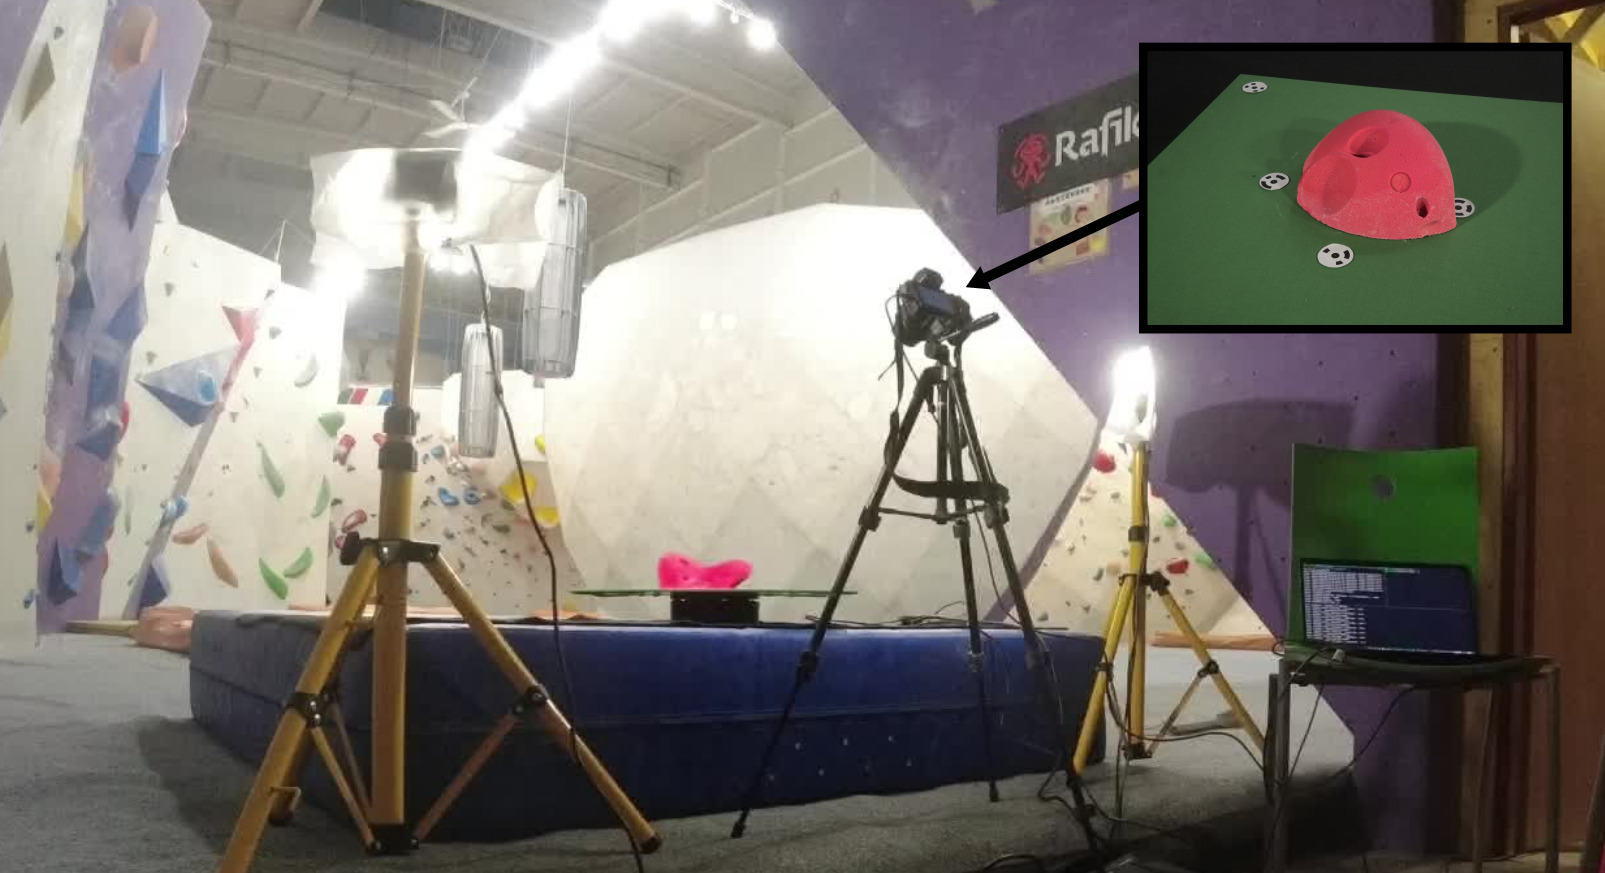
\includegraphics[width=\columnwidth]{images/setup/setup.png}
	\caption{An image of the setup during scanning, including the taken image. f-stop: 22, focal length: \SI{38}{\milli\meter}, ISO: 320, exposure time: \SI{1}{\second}.}
	  
	\label{fig:setup}
\end{figure}

\subsection{Dual texture holds}\label{sec:dual}
Glossy surfaces are a problematic type of surfaces for photogrammetry, since the angle under which they are viewed changes their appearance due to light reflections.
This problem is realized in „dual-texture“ holds which, as the name suggests, contain two textures -- a mate texture that is meant for the climber to hold (or step) onto, and the glossy texture which is usually not.

A standard way of dealing with glossy surfaces is to cover them in something that is mate.
While this does solve the problem of model generation, it ruins the texture, because the mate solution is usually opaque, thus requiring another set of images for texturing.

In our case, however, the solution is pretty straightforward -- cover them in climbing chalk (figure \ref{fig:chalk}).
Since it is mate, it reduces the reflections of the glossy surface and provides additional feature points, making it easier for the photogrammetry software to reconstruct the model.
Additionally, since climbing chalk will be applied to the holds by climber during regular usage anyway, there is no need to obtain more images for texturing.

It is worth noting that this solution is not perfect -- since the chalk doesn't cover the hold entirely, some reflections persist and can introduce model inaccuracies.
In such cases, manual modelling using Blender to reconstruct the missing hold parts is required.

The quality could be further improved by using laser scanning, which handles glossy surfaces better than using images only.

\begin{figure}[t]
	\centering
	\subfloat{{\includegraphics[height=2.5cm]{images/holds/1.png} }}%
	\hfill
	\subfloat{{\includegraphics[height=2.5cm]{images/holds/4.png} }}%
	\hfill
	\subfloat{{\includegraphics[height=2.5cm]{images/holds/3.png} }}%
	\caption{Example of holds with chalk applied. Some reflections are still visible, but they are not as pronounced as with no chalk applied.}%
	\label{fig:chalk}
\end{figure}

\subsection{Hold metadata}
After all models have been generated, a \verb|yaml| metadata file is created for storing their properties.
It is a dictionary, with keys being the hold models and the attributes their properties.
The specification of a single item is as follows:

\begin{minted}{yaml}
<the first 12 characters of the sha256sum of model data>:
  color: [<name>, <hex value>]                 # strings
  type: <the type of hold>                     # string
  manufacturer: <the name of the manufacturer> # string
  labels: [<list>, <of>, <custom>, <labels>]   # strings
  volume: <a float volume of the hold>         # float
  date: <the date the hold model was created>  # datetime
\end{minted}

All of the specified attributes are optional.
Some of them (like volume and date) are automatically inferred, while others have to be added manually.
The first 12 characters of the hashsum were chosen for readability purposes and because millions of holds would be required for a reasonable chance of collision\footnote{Since there are 16 symbols, the total pool of hashes is $N = 16^{12}$. We'll take $n = 10\ 000$ as the maximum number of holds. The chance of collision is inverse to there not being one in the first $n$ holds, which can be calculated as $1 - \prod_{i = 1}^{n} \frac{N - i}{N} \approx 1.77 \cdot 10^{-7}$, which is more than reasonable.}.

\section{Editor implementation}
The editor has been created using the Unity editor, with the majority of the codebase being written in C\#.
While other options exist, such as Unreal Engine and Godot, Unity was chosen due to the author's experience with developing games using it, along with a large ecosystem of packages that could be used to simplify the implementation and allow for rapid prototyping.

Using this ecosystem, a number of freely available packages were used (with minor code modifications), namely

\begin{itemize}
	\item \textbf{Quick Outline} \cite{quickoutline} -- object outline creator,
	\item \textbf{Runtime OBJ Importer} \cite{objimport} -- an \verb|.obj| file importer and
	\item \textbf{Unity Standalone File Browser} \cite{unitystandalonefilebrowser} -- a cross-platform file browser.
\end{itemize}

The editor code is open-source and cross-platform (Mac, Windows, Linux), with newest versions being available at the \href{https://github.com/Climber-Tools/Cled/releases}{project releases page}.

\subsection{Movement}
Movement is implemented using keyboard in a way commonly used in 3D programs.
The arrow or \verb|WSAD| keys provide left, right, forward and backward movement, while the \verb|Space| and \verb|Shift| keys allow flying up and down.

Physics and gravity are also implemented, with the character being pulled to the ground when not flying, and colliding with both the wall and the holds.

\subsection{Wall and hold format}
For the editor to correctly load the scene, it expects the wall and holds to be in the \verb|obj| file format, possibly with a \verb|mtl| file and a bitmap texture.
It has specific requirements on naming and location of the files which differs slightly from Clis.
This is because the editor uses only a subset of the files generated from Clis along with a few that Clis doesn't generate.
To make things easier, the editor contains a Python script to automatically import models from Clis and generate the missing files, which are preview images and preview videos.

The wall can also contain a \verb|yaml| metadata file for wall-specific things, namely the route grades, the names of the setters and which zone the route is located in.
This is to simplify editing route properties by selecting the right option from a dropdown, instead of having to manually type it in.
Here is an example of one such file:

\begin{minted}{yaml}
Grades: ["black", "purple", "red", "salmon", "blue", "yellow"]
Setters: ["Danny", "Bert"]
Zones: ["1", "2", "3", "4", "5"]
\end{minted}

\subsection{Modes}
The editor contains three modes in which can operate, with the current mode being always displayed in the top right.
While this might seem like an implementation detail, it is important for user documentation and general usage, because the user always knows which state the editor is in.
An obvious inspiration is the Vim text editor, which makes the mode distinction similarly apparent.

The modes are the following:

\begin{itemize}
	\item \textbf{NORMAL} -- the mode the user is normally in; hovering highlights holds, which can be either picked up or selected.
	\item \textbf{HOLDING} -- the mode in which the user is holding a specific hold and can place it, or switch to the next one from the selection.
	\item \textbf{ROUTE} -- the mode in which the user is modifying the selected route by adding/removing new holds, or modifying route parameters.
\end{itemize}

\subsection{Hold selection}
Quickly selecting which holds to place on the wall is crucial for effective virtual route setting, because it dictates the time the route setting takes.
The editor contains a menu (accessed via pressing either \verb|Tab| or \verb|Q|) from which a subset of holds can be filtered and cycled while editing.

Filtering holds can be done by selecting a specific hold color, type, manufacturer, or custom hold label.
By default, the currently filtered holds are also sorted first by their color, then by their type and finally by their volume.
Additionally, hovering on each of the menu items rotates them around, which is useful when the static hold image isn't descriptive enough.

TODO: obrázek UI


\subsection{Import and Export}
The import and export format for the project files is a human-readable \verb|yaml| file containing information about the state of the holds, routes, paths to the models and other metadata.
This makes it easy to be used in other applications (both for viewing and modification), since it is well readable and parseable.
Here is how the format looks like:

\begin{minted}{yaml}
Version: 1.0 # Editor version (for compatibility reasons)

Player: # player settings
  Light: false # whether the player's light is on
  Position: # the player position as a vector
    x: 4.66010237
    y: 1.93126345
    z: -8.63198185
  Orientation: # the player orientation (up/down, left/right)
    x: 35.8053398
    y: 123.996086
  Flying: false # whether the player is currently flying

WallModelPath: /home/tom/Wall/wall.obj
HoldModelsPath: /home/tom/Holds

Holds: # a dictionary of hold instances
  f21cde933ad9: # a unique ID for the hold instance
    BlueprintId: 4bdff2704462 # an ID of the hold model
    State:
      Position: # the position of the hold in space
        x: 1.20504105
        y: 0.378549755
        z: -7.67928696
    Normal: # the normal of the hold, away from the wall
        x: 0.994500279
        y: 0.0156783238
        z: 0.103554823
      Rotation: 0 # the hold rotation about the normal
  0436ff53a1d8:
    BlueprintId: 4bdff2704462
    State:
      Position:
        x: 1.46525836
        y: 0.472094655
        z: -8.19389153
      Normal:
        x: 0.752805889
        y: -0.0226488542
        z: 0.657852829
      Rotation: 1.21387374

Routes: # a list of routes
- Name: A very nice route
  Grade: blue
  Zone: 3
  Setter: Danny
  HoldIDs: # which hold instances the route contains
  - 0436ff53a1d8
  - f21cde933ad9

StartingHoldIDs: # a list of starting holds
- f21cde933ad9

EndingHoldIDs: # a list of ending holds
- 0436ff53a1d8

SelectedHoldBlueprintIDs: # a list of currently selected holds
- f21cde933ad9
- 0436ff53a1d8

Lights: # a list of point lights around the wall
  Positions:
  - x: 3.71035504
    y: 3.53241396
    z: -7.11679459
  - x: 5.59678602
    y: 3.53241396
    z: -3.97351503
  Intensity: 0.2 # how strong they are
  ShadowStrength: 0.2 # how hard their shadows are

CaptureSettings: # image capture settings
  ImagePath: /home/tom/Pictures # captured images path
  ImageSupersize: 2 # captured images resolution scaling
\end{minted}

\subsection{Capturing images}
The editor contains functionality for capturing the current image of the wall.
This can be done anywhere in the editor by either selecting the option from the toolbar, or by pressing \verb|Ctrl+P|.
The image is then saved to the default system „Pictures“ folder, unless configured otherwise in the settings.

TODO: obrázek UI

\subsection{Lighting}
Since each wall has different lighting needs and specifying them in the wall metadata would be too impractical, the editor supports placing lights on the current player position (and removing them).
This can be done either from the \verb|Lighting| section of the toolbar, or by using \verb|F| to toggle the player lighting and \verb|Ctrl+F| to place one at the player position.

TODO: obrázek UI

\chapter{Results and discussion}

You should have a separate chapter for presenting your results (generated by the stuff described previously, in our case in \cref{chap:math}). Remember that your work needs to be validated rigorously, and no one will believe you if you just say that `it worked well for you'.

Instead, try some of the following:
\begin{itemize}
\item State a hypothesis and prove it statistically
\item Show plots with measurements that you did to prove your results (e.g. speedup). Use either \texttt{R} and \texttt{ggplot}, or Python with \texttt{matplotlib} to generate the plots.\footnote{Honestly, the plots from \texttt{ggplot} look \underline{much} better.} Save them as PDF to avoid printing pixels (as in \cref{fig:f}).
\item Compare with other similar software/theses/authors/results, if possible
\item Show example source code (e.g. for demonstrating how easily your results can be used)
\item Include a `toy problem' for demonstrating the basic functionality of your approach and detail all important properties and results on that
\item Include clear pictures of `inputs' and `outputs' of all your algorithms, if applicable
\end{itemize}

\begin{figure}
\centering
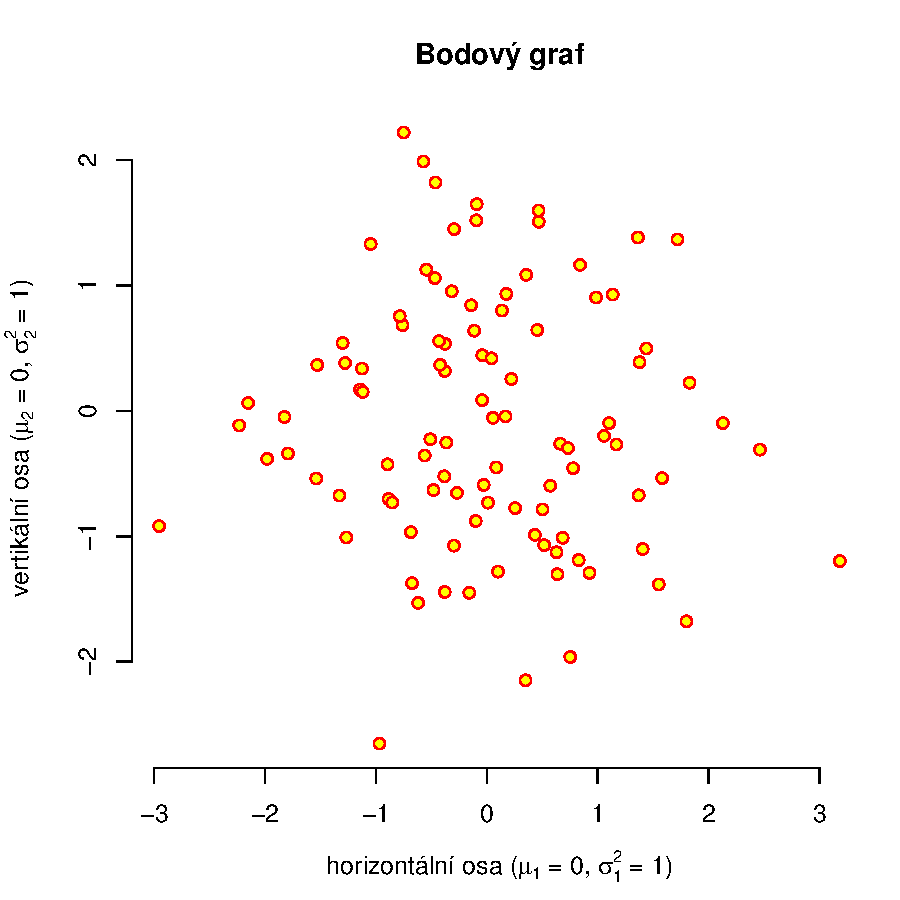
\includegraphics[width=.6\linewidth]{img/ukazka-obr01.pdf}
\caption{This caption is a friendly reminder to never insert figures ``in text,'' without a floating environment, unless explicitly needed for maintaining the text flow (e.g., the figure is small and developing with the text, like some of the centered equations, as in \cref{thm:y}). All figures \emph{must} be referenced by number from the text (so that the reader can find them when he reads the text) and properly captioned (so that the reader can interpret the figure even if he looks at it before reading the text --- reviewers love to do that).}
\label{fig:f}
\end{figure}

It is sometimes convenient (even recommended by some journals, including Cell) to name the results sub-sections so that they state what exactly has been achieved. Examples follow.

\section{SuperProgram is faster than OldAlgorithm}
\subsection{Scalability estimation}
\subsection{Precision of the results}
\section{Weird theorem is proven by induction}
\section{Amount of code reduced by CodeRedTool}
\subsection{Example}
\subsection{Performance on real codebases}
\section{\sloppy NeuroticHelper improves neural network learning}

\section{Graphics and figure quality}

No matter how great the text content of your thesis is, the pictures will always catch the attention first. This creates the very important first impression of the thesis contents and general quality. Crucially, that also decides whether the thesis is later read with joy, or carefully examined with suspicion.

Preparing your thesis in a way such that this first impression gets communicated smoothly and precisely helps both the reviewer and you: the reviewer will not have a hard time understanding what exactly you wanted to convey, and you will get a better grade.

Making the graphics `work for you' involves doing some extra work that is often unexpected. At the same time, you will need to fit into graphics quality constraints and guidelines that are rarely understood before you actually see a bad example. As a rule of thumb, you should allocate at least the same amount of time and effort for making the figures look good as you would for writing, editing and correcting the same page area of paragraph text.

\subsection{Visualize all important ideas}
The set of figures in your thesis should be comprehensive and complete. For all important ideas, constructions, complicated setups and results there should be a visualization that the reader can refer to in case the text does not paint the `mental image' sufficiently well. At the bare minimum, you should have at least 3 figures (roughly corresponding to the 3 chapters) that clearly and unambiguously show:
\begin{enumerate}
\item the context of the problem you are solving, optionally with e.g.~question marks and exclamation marks placed to highlight the problems and research questions
\item the overall architecture of your solution (usually as a diagram with arrows, such as in \cref{fig:schema}, ideally with tiny toy examples of the inputs and outputs of each box),
\item the advancement or the distinctive property of your solution, usually in a benchmark plot, or as a clear demonstration and comparison of your results.
\end{enumerate}

\subsection{Make the figures comprehensible}
The figures should be easily comprehensible. Surprisingly, that requires you to follow some common ``standards'' in figure design and processing. People are often used to a certain form of the visualizations, and (unless you have a very good reason) deviating from the standard is going to make the comprehension much more complicated. The common standards include the following:
\begin{itemize}
  \item caption everything correctly, place the caption at an expectable position
  \item systematically label the plots with `main' titles (usually in boldface, above the plot), plot axes, axis units and ticks, and legends
  \item lay out the diagrams systematically, ideally follow a structure of a bottom-up tree, a left-to-right pipeline, a top-down layered architecture, or a center-to-borders mindmap
  \item {use colors that convey the required information correctly \par\footnotesize Although many people carry some intuition for color use, achieving a really correct utilization of colors is often very hard without previous experience in color science and typesetting. Always remember that everyone perceives color hues differently, therefore the best distinction between the colors is done by varying lightness of the graphics elements (i.e., separating the data by dark vs.~light) rather than by using hues (i.e., forcing people to guess which one of salmon and olive colors means ``better''). Almost 10\% of the population have their vision impaired by some form of color vision deficiency, most frequently by deuteranomaly that prevents interpretation of even the most `obvious' hue differences, such as green vs.~red. Finally, printed colors look surprisingly different from the on-screen colors. You can prevent much of these problems by using standardized palettes and well-tested color gradients, such as the ones from ColorBrewer\footnote{\url{https://colorbrewer2.org}} and ViridisLite\footnote{\url{https://sjmgarnier.github.io/viridisLite/}}. Check if your pictures still look good if converted to greyscale, and use a color deficiency simulator to check how the colors are perceived with deuteranomaly.}
\end{itemize}

Avoid large areas of over-saturated and dark colors:
\begin{itemize}
  \item under no circumstances use dark backgrounds for any graphical elements, such as diagram boxes and tables --- use very light, slightly desaturated colors instead
  \item avoid using figures that contain lots of dark color (as a common example, heatmaps rendered with the `magma' color palette often look like huge black slabs that are visible even through the paper sheet, thus making a dark smudge on the neighboring page)
  \item increase the brightness of any photos to match the average brightness of the text around the figure
\end{itemize}

Remember to test your figures on other people --- usually, just asking `What do you think the figure should show?' can help you debug many mistakes in your graphics. If they think that the figure says something different than what you planned, then most likely it is your figure what is wrong, not the understanding of others.

Finally, there are many magnificent resources that help you arrange your graphics correctly. The two books by Tufte~\cite{tufte1990envisioning,tufte1983visual} are arguably classics in the area. Additionally, you may find many interesting resources to help you with technical aspects of plotting, such as the \texttt{ggplot}-style `Fundamentals' book by~\citet{wilke2019fundamentals}, and a wonderful manual for the TikZ/PGF graphics system by~\citet{tantau2015tikz} that will help you draw high-quality diagrams (like the one in~\cref{fig:schema}).

\section{What is a discussion?}
After you present the results and show that your contributions work, it is important to \emph{interpret} them, showing what they mean in the wider context of the thesis topic, for the researchers who work in the area, and for the more general public, such as for the users.

Separate discussion sections are therefore common in life sciences where some ambiguity in result interpretation is common, and the carefully developed intuition about the wider context is sometimes the only thing that the authors have. Exact sciences and mathematicians do not need to use the discussion sections as often. Despite of that, it is nice to position your output into the previously existing environment, answering:
\begin{itemize}
\item What is the potential application of the result?
\item Does the result solve a problem that other people encountered?
\item Did the results point to any new (surprising) facts?
\item How (and why) is the approach you chose different from what the others have done previously?
\item Why is the result important for your future work (or work of anyone other)?
\item Can the results be used to replace (and improve) anything that is used currently?
\end{itemize}

If you do not know the answers, you may want to ask the supervisor. Also, do not worry if the discussion section is half-empty or completely pointless; you may remove it completely without much consequence. It is just a bachelor thesis, not a world-saving avenger thesis.

\chapwithtoc{Conclusion}\label{sec:conclusion}
Clis and Cled have been successfully tested on the Smíchoff bouldering wall, creating a dataset of 119 holds (in 4 hours), the textured wall model (in 5 hours) and virtually setting a number of routes from the wall (see figure \ref{fig:capture}).

% hack to include this in TOC
\setcounter{secnumdepth}{0}

\section{Future developments}
Future developments include implementing a web interface and a mobile application, so the exported routes can be interacted with by regular users.
Such interface should support the ideas outlined in the introduction, such as route filtering, liking/disliking and send videos.

Additional features that were beyond the scope of this project but will be implemented in the future are automatic hold placement from a photo of the wall using SIFT (described in section \ref{ch:fext}), „snapping to hole“ for holds that can only be placed in specific ways and a large number of quality-of-life improvements and bugfixes.
Laser scanning is also a potential improvement for model generation.
Furthermore, the option of using VR to increase setting efficiency will be explored.

Another possible use for the data produced by Clis and Cled is for the purposes of simulating the movements of a climber on the wall.

The end goal is to provide Clis and Cled as a service for climbing gyms all over the world, so climbers have an easier time picking where to go climbing and can better find people to go climbing with, and routesetters have an easier time of building higher-quality routes.

\section{Routesetter feedback}
To test the editor implementation functionality, two of Smíchoff's routesetters were asked to provide feedback regarding the editor usage.
The feedback was positive, with the main conclusion being that the editor would be suitable for climbing gyms with lower frequency of wall changes, since the editor adds a non-trivial overhead that smaller climbing gyms could not sustain.

% hack to include this in TOC
\setcounter{secnumdepth}{3}


\ifEN
\chapwithtoc{Bibliography}
\else
\chapwithtoc{Seznam použité literatury}
\fi

\printbibliography[heading=none]


\appendix
\chapter{Generating markers}

The markers were calculated and generated using Matthew Petroff's Python scripts, available under the CC0 1.0 license.

To calculate the number of valid targets run \verb|find_codes.py|. To generate them in the PDF rormat, run \verb|create_target_sheets.py|. Note that to change the parameters of the PDF, you must directly edit the top of the source code.

% TODO: include the code?

%The program can be used as a C++ library, the simplest use is demonstrated in \cref{lst:ex}. A demonstration program that processes demonstration data is available in directory \verb|demo/|, you can run the program on a demonstration dataset as follows:
%\begin{Verbatim}
%cd demo/
%./bin/cool_process_data data/demo1
%\end{Verbatim}
%
%After the program starts, control the data avenger with standard \verb-WSAD- controls.
%
%\begin{listing}
%\begin{lstlisting}
%#include <CoolSoft.h>
%#include <iostream>
%
%int main() {
%	int i;
%	if(i = cool::ProcessAllData()) // returns 0 on error
%		std::cout << i << std::endl;
%	else
%		std::cerr << "error!" << std::endl;
%	return 0;
%}
%\end{lstlisting}
%\caption{Example program.}
%\label{lst:ex}
%\end{listing}


% if your attachments are complicated, describe them in a separate appendix
%\include{attachments}

\openright
\end{document}
